\question 在一棵度数为4的树T中,若有20个度为4的结点,10个度为3的结点,1个度为2的结点,10个度为1的结点,则树T的叶结点个数是(
)
\par\twoch{41}{\textcolor{red}{82}}{113}{122}
\begin{solution}设树的总结点数为n,由于树T的度为4,故树T只能有度为0、1、2、3、4的结点。设ni为度为i的结点数。n=n0+n1+n2+n3+n4(其中n0即为叶结点的个数)。在一棵树中,度之和=结点数-1=n-1。又度之和=1×n1+2×n2+3×n3+4×n4=1×10+2×1+3×10+4×20=122。即n-1=122,得到n=123。n0=n-n1-n2-n3-n4=123-10-1-10-20=82。
【总结】 树的度之和=分支数=结点数减1。
\end{solution}
\question 已知三叉树T中6个叶结点的权分别是2,3,4,5,6,7,T的带权(外部)路径长度最小是(
~)
\par\twoch{27}{\textcolor{red}{46}}{54}{56}
\begin{solution}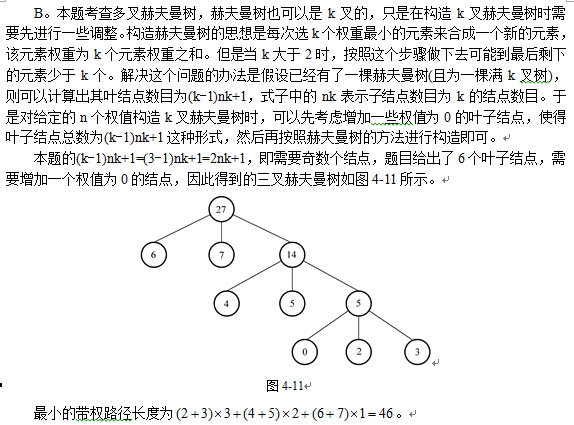
\includegraphics[width=3.33333in,height=2.64583in]{computerassets/e9d6a97804263e5cf8b47d8cd8b830dd.jpeg}
\end{solution}
\question (北京航空航天大学,2004年)若一棵度为7的树有8个度为1的节点,有7个度为2的节点,有6个度为3的节点,有5个度为4的节点,有4个度为5的节点,有3个度为6的节点,有2个度为7的节点,该树一共有(
)个叶子节点
\par\twoch{35}{28}{77}{\textcolor{red}{78}}
\begin{solution}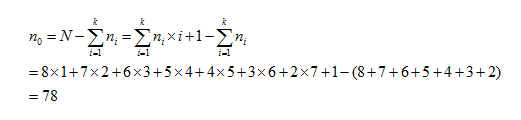
\includegraphics[width=5.42708in,height=1.25000in]{computerassets/8640ea38b1bda9fc51d44e6d23929ade.png}
\end{solution}
\question (南京邮电大学,2005年)一棵三叉树中,已知度为3的节点个数等于度为2的结点数,且树中叶子节点的数目为13,则度为2的节点数目为(
)
\par\twoch{\textcolor{red}{4}}{2}{3}{5}
\begin{solution}首先,我们必须知道总结点数=分支数+1,假设度为3的节点有x个,度为2的节点有y个,度为1的节点有z个,度为0的节点有m个,那么有x+y+z+m=3x+2y+z+1,将m=13,x=y代入,可得x=4。
\end{solution}
